\section{Auswertung}
\label{sec:Auswertung}
\subsection{Vorbereitung}
Vor dem Messen der Fallzeiten werden die Kenngrößen der beiden Glaskugeln bestimmt. Dabei ergeben sich für die beiden Kugeln die folgenden Werte:

\begin{table}[h]
    \centering
    \caption{Kenngrößen der Glaskugeln.}
    \label{tab:mess_klKugel_raum}
    \begin{tabular}{c c c c}
        \toprule
        & {Gewicht $m\:/\:\si{\gram}$} & {Durchmesser $d\:/\:\si{\milli\meter}$} & Dichte $\rho\:/\:\si{\kilo\gram\per\meter}$\\
        \midrule % nicht sicher, warum hier die Dichte so deutlich unterschiedlich ist. Auch nicht sicher, ob das in die Tabelle sollte. da wir aber damit rechnen, dürfte das wohl nicht schaden.
        Kleine Kugel & 4.4531 & 15.60 & 2416.5 \\
        Große Kugel  & 4.9528 & 15.76 & 2240.2 \\
        \bottomrule
    \end{tabular}    
\end{table}
\subsection{Viskositäten}
\subsubsection{Kleine Kugel, Raumtemperatur}
Es werden zehn Messungen bei Raumtemperatur für die kleine Glaskugel vorgenommen.

\begin{table}[h]
    \centering
    \caption{Fallzeiten der kleinen Kugel bei Raumtemperatur.}
    \label{tab:mess_klKugel_raum}
    \begin{tabular}{c c}
        \toprule
        \multicolumn{2}{c}{Fallzeit $t\:/\:\si{\second}$} \\
        \midrule
        12.40 & 12.17 \\
        12.36 & 12.35 \\
        12.31 & 12.09 \\
        12.43 & 12.35 \\
        12.57 & 12.52 \\
        \bottomrule
    \end{tabular}    
\end{table}

Hierbei sind die bereits erwähnten Bedingungen, insbesondere aber die Blasenfreiheit genau zu beachten.
Es errechnet sich eine gemittelte Fallzeit von

\begin{equation*}
    \text{Temperatur }\SI{23.5}{\celsius} \qquad\qquad \text{Fallzeit }\SI{12.355\pm0.137}{\second}.
\end{equation*}

Über Gleichung \eqref{eqn:exp_visk} lässt sich dann mit gegebener Gerätekonstante \\
$K_{kl} = \SI{0.07640e-6}{\pascal\meter\cubed\per\kilo\gram}$ die Viskosität berechnen zu
$\eta_{kl} = \SI{1173\pm13e-6}{\kilo\gram\per\meter\per\second}$. 

\subsubsection{Große Kugel, dynamische Temperatur}
Für die große Kugel werden ebenfalls zehn Messwerte aufgenommen. Im Anschluss wird die Temperatur um wenige Grade erhöht und die Messungen wiederholt.
Es folgen insgesamt neun Temperaturerhöhungen, wodurch 100 Messwerte für die große Kugel aufgenommen werden.


Da auch die große Glaskugel bei Raumtemperatur untersucht wird, kann mit $K_{kl}$ und der nun bekannten Viskosität $\eta_{kl}$ die Gerätekonstante $K_{gr} = \SI{8.99\pm0.11e-09}{\pascal\meter\cubed\per\kilo\gram}$ über \eqref{eqn:exp_visk}
ausgerechnet werden.
Im Weiteren wird die Viskosität des Wassers bei veränderter Temperatur ermittelt.

\begin{table}[h]
    \centering
    \caption{Mittlere Fallzeiten und Viskosität der großen Kugel.}
    \label{tab:mess_grKugel_dyn}
    \begin{tabular}{c c l}
        \toprule
        {Temperatur $T\:/\:\si{\celsius}$} & {Fallzeit $t\:/\:\si{\second}$} & {Viskosität $\eta_{gr}\:/\:\si{\kilo\gram\per\meter\per\second}$} \\
        \midrule
        23.5 & 91.91$\pm$0.53 & $\qquad\qquad$   1172$\pm$13 \\
        31.5 & 71.08$\pm$0.81 & $\qquad\qquad\;\;$  908$\pm$15 \\
        35.0 & 67.22$\pm$1.12 & $\qquad\qquad\;\;$  860$\pm$17 \\
        39.0 & 61.66$\pm$0.30 & $\qquad\qquad\;\;$  789$\pm$10 \\
        42.0 & 57.57$\pm$0.30 & $\qquad\qquad\;\;$  737$\pm$10 \\
        46.0 & 53.45$\pm$0.33 & $\qquad\qquad\;\;$  685$\pm$ 9 \\
        51.0 & 49.01$\pm$0.48 & $\qquad\qquad\;\;$  629$\pm$10 \\
        55.0 & 45.80$\pm$0.25 & $\qquad\qquad\;\;$  589$\pm$ 8 \\
        60.0 & 43.04$\pm$0.31 & $\qquad\qquad\;\;$  554$\pm$ 8 \\
        64.0 & 40.33$\pm$0.12 & $\qquad\qquad\;\;$  520$\pm$ 6 \\
        \bottomrule
    \end{tabular}    
\end{table}

\begin{figure}
    \centering
    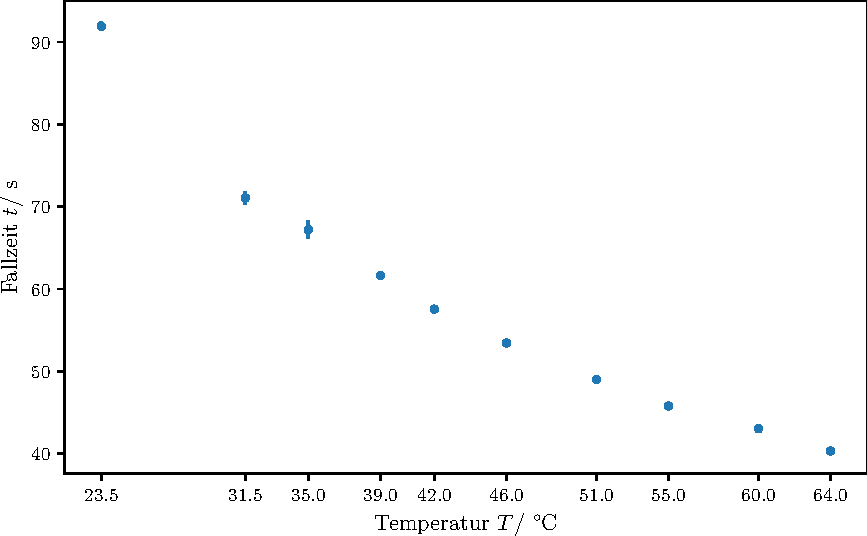
\includegraphics{plots/avg_gr.pdf}
    \caption{Gemittelte Fallzeiten der großen Kugel.}
    \label{fig:mittl_fall_gr}
\end{figure}

Ein Vergleich mit der Literatur\cite{taschenbuch} zeigt, dass die Werte in einem plausiblen Bereich liegen.\footnote{Für einen genaueren Vergleich wurde eine Ausgleichsfunktion der Form $(a * 1/(x-b)) + c$ mit $a = 49737, b = -26, c = -93$ über 13 Literaturwerte gelegt.}

\begin{table}[h]
    \centering
    \caption{Vergleich der Viskositäten $\eta_{gr}$ mit Literaturwerten.}
    \label{tab:mess_grKugel_theo}
    \begin{tabular}{c l c}
        \toprule
        {Temperatur $T\:/\:\si{\celsius}$} & {$\eta_{gr}\:/\:\si{\kilo\gram\per\meter\per\second}$} & {$\eta_{theo}\:/\:\si{\kilo\gram\per\meter\per\second}$} \\
        \midrule
        23.5 & $\:$   1172$\pm$13 & 908 \\
        31.5 & $\;\;$  908$\pm$15 & 769 \\
        35.0 & $\;\;$  860$\pm$17 & 720 \\
        39.0 & $\;\;$  789$\pm$10 & 670 \\
        42.0 & $\;\;$  737$\pm$10 & 636 \\
        46.0 & $\;\;$  685$\pm$ 9 & 596 \\
        51.0 & $\;\;$  629$\pm$10 & 551 \\
        55.0 & $\;\;$  589$\pm$ 8 & 519 \\
        60.0 & $\;\;$  554$\pm$ 8 & 484 \\
        64.0 & $\;\;$  520$\pm$ 6 & 458 \\
        \bottomrule
    \end{tabular}    
\end{table}

\begin{figure}
    \centering
    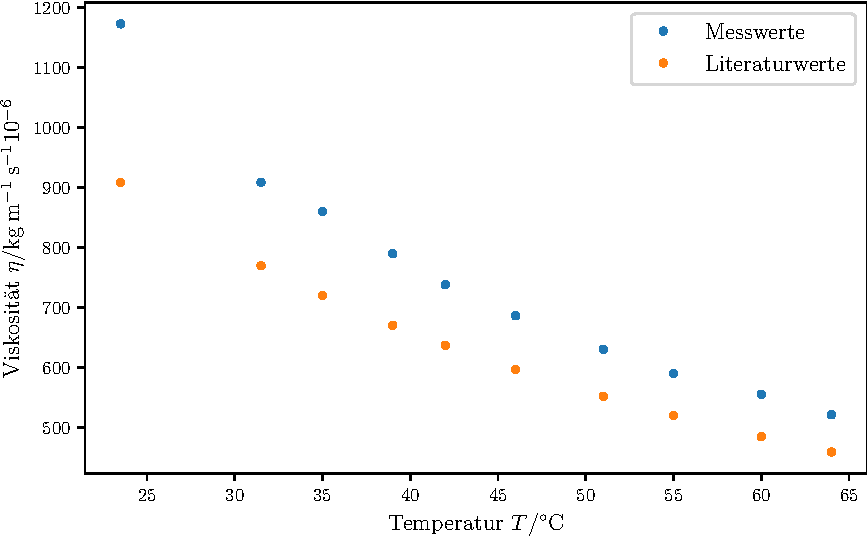
\includegraphics{plots/visk_theo.pdf}
    \caption{Literatur- und Messwerte der Viskosität $\eta_{gr}$.}
    \label{fig:lit_mess_gr}
\end{figure}


\FloatBarrier
\subsection{Reynoldszahl}
Die Reynoldszahl gibt Aufschluss darüber, ob eine Ströumung turbulent oder laminar ist. Wie in der Theorie bereits erwähnt gibt es die kritische Reynoldszahl,
welche Aufschluss darüber gibt, ob eine Strömung ihren Zustand zwischen den genannten Eigenschaften ändert.
Für die in diesem Versuch verwendete Apparatur ist $\symup{R_{crit}} \approx 2300$.\cite{taschenbuch}
Zunächst werden die Fallgeschwindigkeiten bestimmt, um die Reynoldszahl über \eqref{eqn:reynold} auszurechnen. Dafür wird eine Falldistanz von $x = \SI{100}{\milli\meter}$ verwendet.
Es ergibt sich $v_{kl} = \SI{8.09\pm0.09}{\milli\meter\per\second}$.
Für die charakteristische Länge $L$ werden die Durchmesser der Glaskugeln verwendet. Aus \eqref{eqn:reynold} errechnen sich die Reynoldszahlen zu 
$R_{kl} = 107.4\pm2.4$. Die Werte der großen Kugel sind in der nachstehenden Tabelle aufgeführt.

\begin{table}[h]
    \centering
    \label{tab:geschw_gr_rey}
    \caption{Fallgeschwindigkeiten und Reynoldszahlen der großen Kugel.}
    \begin{tabular}{c}
        \toprule
        {$v_{gr}\:/\:\si{\milli\meter\per\second}$} \\
        \midrule
        1.088$\pm$0.006 \\
        1.406$\pm$0.016 \\
        1.487$\pm$0.024 \\
        1.621$\pm$0.007 \\
        1.736$\pm$0.009 \\
        1.870$\pm$0.011 \\
        2.040$\pm$0.020 \\
        2.182$\pm$0.012 \\
        2.323$\pm$0.016 \\
        2.479$\pm$0.007 \\
        \bottomrule
    \end{tabular}
    $\qquad\qquad$
    \begin{tabular}{c}
        \toprule
        {$R_{gr}$} \\
        \midrule
        14.5$\pm$0.1 \\
        24.2$\pm$0.6 \\
        27.0$\pm$0.9 \\
        32.1$\pm$0.5 \\
        36.7$\pm$0.6 \\
        42.5$\pm$0.7 \\
        50.4$\pm$1.1 \\
        57.5$\pm$0.9 \\
        64.8$\pm$1.2 \\
        73.6$\pm$1.0 \\
        \bottomrule
    \end{tabular}     
\end{table}

\begin{table}[h]
    \centering
    \caption{Fallzeiten der großen Kugel bei steigender Temperatur.}
    \label{tab:mess_grKugel_dyn}
    \begin{tabular}{c c c c c c}
        \toprule
        {Temperatur $T\:/\:\si{\celsius}$} & \multicolumn{2}{c}{Fallzeit $t\:/\:\si{\second}$} & {Temperatur $T\:/\:\si{\celsius}$} & \multicolumn{2}{c}{Fallzeit $t\:/\:\si{\second}$} \\
        \midrule
        23.5 & 92.25 & 92.32 & 46.0 & 53.47 & 53.29 \\
             & 91.48 & 91.32 &      & 52.74 & 53.53 \\
             & 91.22 & 91.25 &      & 53.22 & 53.89 \\
             & 92.12 & 91.83 &      & 53.27 & 53.99 \\
             & 92.62 & 92.69 &      & 53.56 & 53.62 \\
                                                    \\
        31.5 & 71.75 & 72.13 & 51.0 & 49.50 & 49.35 \\
             & 71.75 & 71.83 &      & 49.22 & 49.35 \\
             & 70.69 & 71.62 &      & 49.32 & 49.47 \\
             & 71.03 & 70.42 &      & 48.06 & 48.33 \\
             & 69.85 & 69.80 &      & 48.93 & 48.59 \\
                                                    \\
        35.0 & 69.22 & 69.39 & 55.0 & 46.16 & 45.81 \\
             & 67.31 & 67.01 &      & 45.98 & 45.84 \\
             & 66.88 & 66.92 &      & 46.00 & 45.14 \\
             & 67.17 & 66.25 &      & 45.84 & 45.76 \\
             & 66.19 & 65.93 &      & 45.84 & 45.72 \\
                                                    \\
        39.0 & 61.90 & 61.91 & 60.0 & 43.38 & 43.09 \\
             & 62.00 & 62.00 &      & 43.17 & 42.54 \\
             & 61.81 & 61.66 &      & 42.53 & 43.51 \\
             & 61.12 & 61.21 &      & 43.00 & 42.81 \\
             & 61.54 & 61.46 &      & 43.18 & 43.26 \\
                                                    \\
        42.0 & 57.37 & 57.87 & 64.0 & 40.53 & 40.34 \\
             & 57.56 & 57.55 &      & 40.19 & 40.24 \\
             & 57.62 & 57.54 &      & 40.28 & 40.28 \\
             & 58.00 & 57.97 &      & 40.46 & 40.48 \\
             & 57.03 & 57.20 &      & 40.16 & 40.42 \\
        \bottomrule
    \end{tabular}    
\end{table}


\FloatBarrier
\subsection{Andrade'sche Gleichung}
Mit \eqref{eqn:andrade} wird die Viskosität temperaturabhängig dargestellt. Um eine Gerade zu erhalten wird die Gleichung in die Form
$\text{ln}(\eta) = \text{ln}(A) + B \cdot \sfrac{1}{T}$ gebracht. Mit einer Ausgleichsgeraden ergeben sich die Werte zu $A = (2.7\pm0.6)\cdot10^{-6}$ und $B = 1932\pm75$.

\begin{figure}[!h]
    \centering
    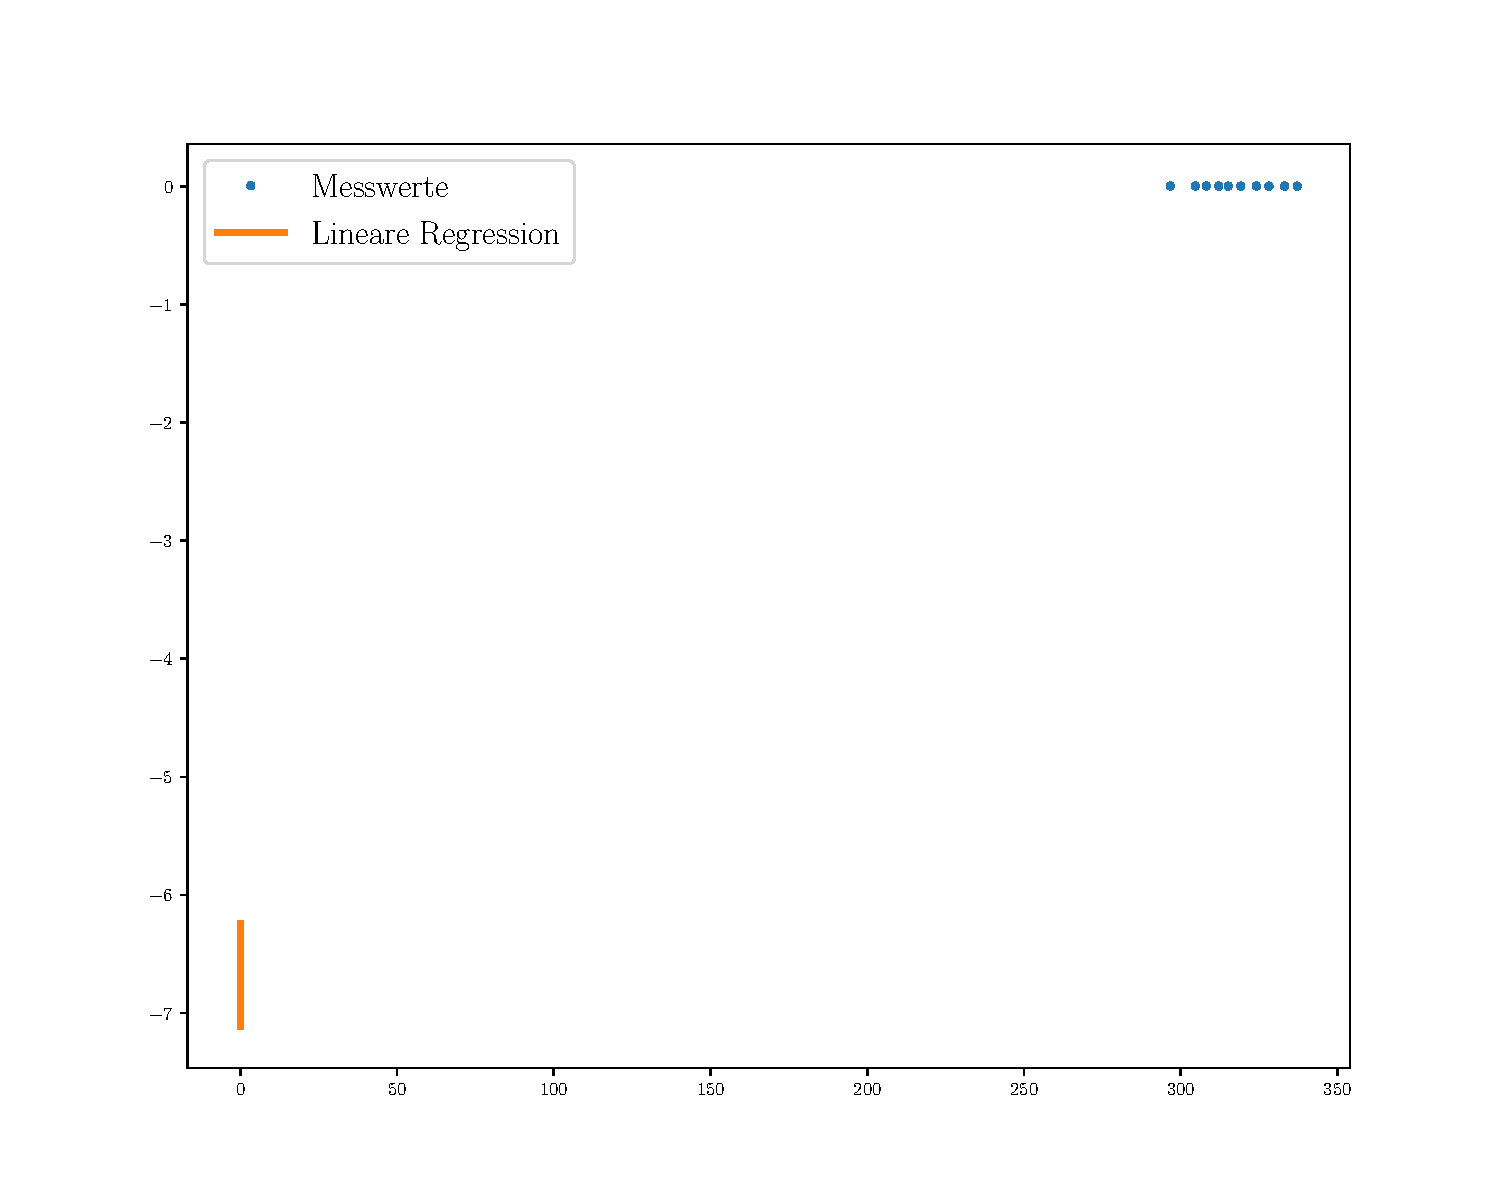
\includegraphics[width=0.9\textwidth]{plots/plot_2.pdf}
    \caption{Lineare Ausgleichsgerade aus der Andrade'schen Gleichung.}
    \label{fig:andrade}
\end{figure}